\def\themis{Themis\xspace}

\chapter{I/O-Efficient Fault Tolerance}
\label{chapter:fault_tolerance}

A key requirement when building scale-out data processing architectures is
allowing them to recover from failures in a manner that is transparent to the
end user. Traditional MapReduce implementations provide fault tolerance by
materializing intermediate data to disk on both sides of a network
transfer. This increases the amount of disk I/O that each MapReduce job must
perform, which fundamentally limits the performance of I/O-bound workloads.

In this chapter, we argue that small and medium clusters -- on which MapReduce
is commonly deployed, and where the likelihood of a failure during a job is low
relative to large-scale clusters -- can benefit from more optimistic forms of
fault tolerance for which the common-case overhead is far lower than
traditional approaches. In particular, we explore the implications of the
job-level fault tolerance approach adopted by Themis in the previous chapter,
and describe an alternative fault tolerance method for Themis that leverages
prior work in scan sharing and eager record-level provenance.


\section{Introduction}

A key requirement and challenge in building scale-out data processing
architectures is allowing them to recover from failures without burdening the
programmer. MapReduce traditionally provides fault tolerance by splitting the
execution of the \map and \reduce functions into a collection of idempotent
\emph{tasks}. Each map task operates over a portion of the input, while each
reduce task operates over records produced by the \map function with a
particular set of keys. When a task fails, it is simply re-executed. We refer
to this method of fault tolerance as ~\emph{task-level fault tolerance}.

A key benefit of this fault tolerance technique is that it is
\emph{proportional}. Generally speaking, this means that the amount of
additional work required to recover from a failure is proportional to the size
of that failure. Proportional fault tolerance techniques work extremely well on
clusters containing thousands of nodes, because failures in those environments
are extremely common and the relative size of each individual failure is
small~\cite{jeff-dean-talk}.

In MapReduce's case, however, proportional fault tolerance comes with a
significant cost; map tasks must materialize their output to their local disks
before transferring that output to reduce tasks. These materializations are
required because, in general, each reduce task needs some of the records
produced by every map task in order to run. Were map tasks to send their
outputs to reduce tasks directly, the loss of the node on which a reduce
task runs would require that map tasks re-compute all data sent to that
task. In I/O-bound applications, the extra materializations required by
task-level fault tolerance can negatively
affect performance.

Many modern MapReduce clusters are ``dense'', in the sense that they pack a
large amount of storage, compute, and network bandwidth into a small number of
racks of servers. In this chapter, we show that in these ``dense'' clusters,
the additional I/O necessitated by task-level fault tolerance often leads to
lower overall job throughput than simply re-running a job if a failure
occurs.

The more optimistic \emph{job-level fault tolerance} employed by \themis in the
previous chapter allows \themis to perform much more aggressive operator
pipelining than task-level fault tolerance can achieve while still maintaining
the 2-IO property. However, job-level fault tolerance precludes running jobs
that take longer than the cluster MTTF to complete, preventing large clusters
(or unusually failure-prone small ones) from running some jobs.  To mitigate
this problem, we present a fault tolerance approach that provides proportional
recovery without imposing additional intermediate data materialization during
failure-free execution. Our main goal in designing this fault tolerance scheme
is to perform as little additional I/O as possible both in common case
operation and during recovery from failure.

Our contributions are as follows:

\begin{enumerate}
  \item We explore the tradeoffs of different levels of fault tolerance in
    ``dense'' clusters.
  \item We modify \themis to allow it to run multiple jobs concurrently, using
    scan sharing~\cite{nova, qptmd, coscan} to reduce the amount of I/O
    required for each job.
  \item Leveraging this multi-tenant capability, we present a fault tolerance
    mechanism that composes previously known techniques to reduce the amount of
    additional I/O needed for recovery at the expense of additional redundant
    computation.
  \item We show how this fault tolerance mechanism can be used to provide
    proportional recovery both from failures of a single disk and an entire
    node. When scan sharing, an eight-node \themis cluster can recover from a
    disk failure with under 5\% overhead.
  \item We compare this approach to approaches based on record-based provenance
    information.
\end{enumerate}

\section{Motivation}
\label{sec:motivation}
\label{sec:assumptions}

In this section, we summarize the argument for replacing task-level fault
tolerance as MapReduce's fault tolerance scheme for ``dense'' clusters. We then
provide an overview of alternative fault approaches used by current data
processing systems.

\subsection{Fault Tolerance for ``Dense'' Clusters}
\label{sec:ft_provenance}

\begin{figure*}[t]
\centering
\begin{subfigure}[t]{0.47\textwidth}
  \centering
  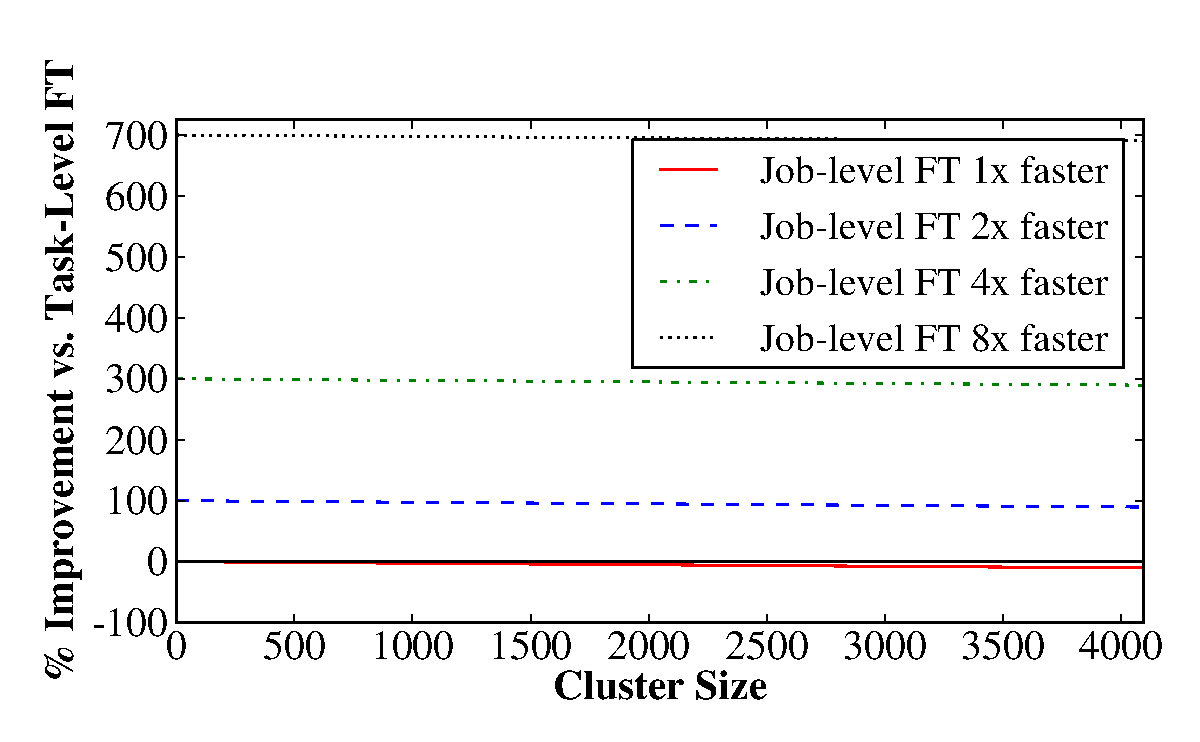
\includegraphics[width=\textwidth]{themis/graphs/analytical_failure_motivation/factor_5min}
  \caption{\label{fig:ft_motivation5} 5-minute job}
\end{subfigure}
\begin{subfigure}[t]{0.47\textwidth}
\centering
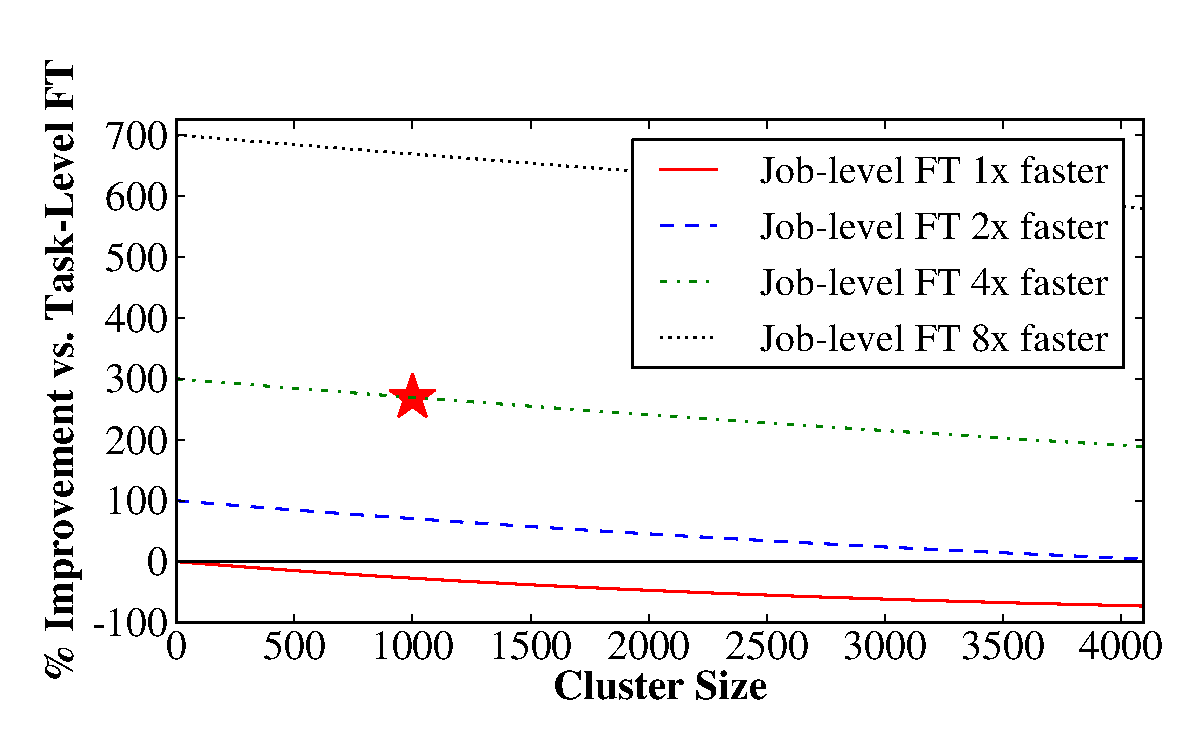
\includegraphics[width=\textwidth]{themis/graphs/analytical_failure_motivation/factor_60min}
\caption{\label{fig:ft_motivation60} 1-hour job (see text below for explanation of marked point)}
\end{subfigure}
\begin{subfigure}[t]{0.47\textwidth}
\centering
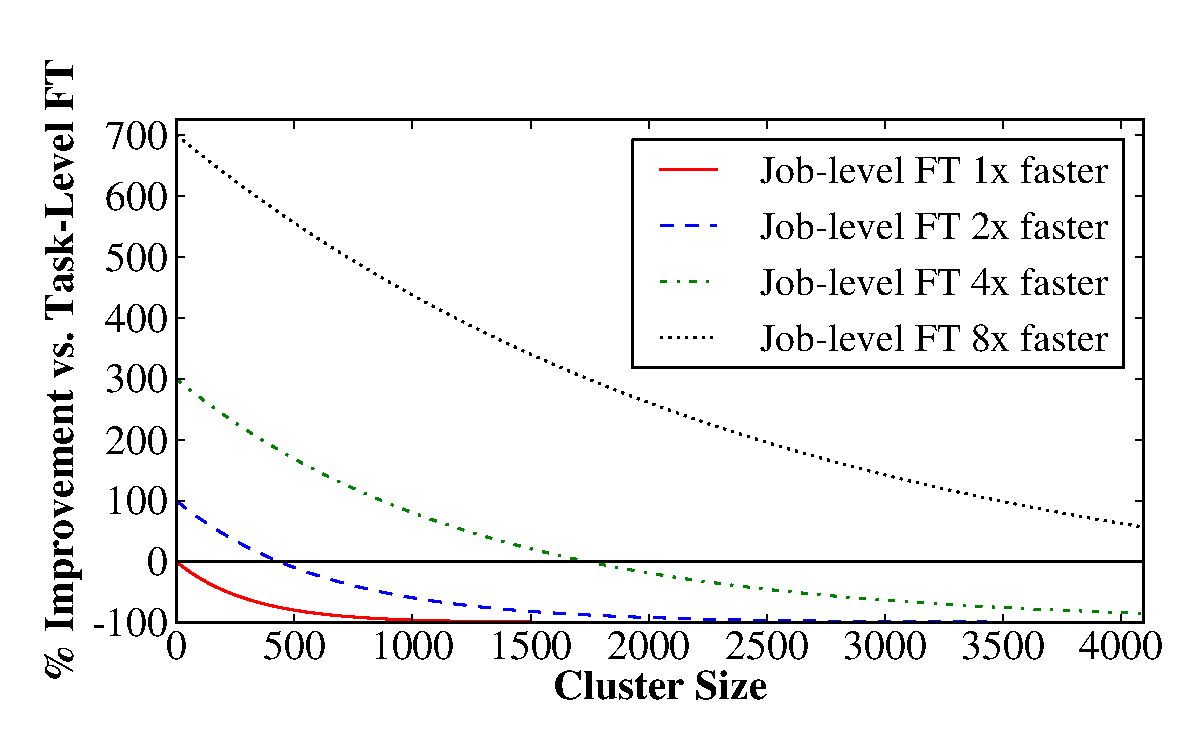
\includegraphics[width=\textwidth]{themis/graphs/analytical_failure_motivation/factor_600min}
\caption{\label{fig:ft_motivation600}10-hour job}
\end{subfigure}
\caption{\label{fig:ft_motivation} A lower-bound of the expected benefit of
  job-level fault tolerance for varying cluster sizes, given
  that an error-free execution of a job with task-level fault tolerance takes
  five minutes (\subref{fig:ft_motivation5}), an hour (\subref{fig:ft_motivation60}),
  or ten hours (\subref{fig:ft_motivation600}) to complete.}
\end{figure*}

Much of MapReduce's architecture is based on the assumption that it is running
on a very large cluster of unreliable machines.  However, a large number of
``Big Data'' clusters do not approach the size of warehouse-scale data centers
like those at Google and Microsoft because moderately-sized clusters (10s of
racks or fewer) are increasingly able to support important real-world problem
sizes.  The storage capacity and number of CPU cores in commodity servers are
both increasing rapidly.  In Cloudera's reference system
design~\cite{ClouderaDellHadoopPlatform}, in which each node has 16 or more
disks, a petabyte worth of 1TB drives fits into just over three racks, or about
60 nodes.  Coupled with the emergence of affordable 10 Gbps Ethernet at the end
host and increasing bus speeds, data can be packed more densely than ever
before while keeping disk I/O as the bottleneck resource.  This implies that
fewer servers are required for processing large amounts of data for I/O-bound
workloads.  We now consider the implications of this increased density on fault
tolerance.

Job-level fault tolerance allows for much more aggressive operator pipelining
than task-level fault tolerance can achieve while still maintaining the 2-IO
property.  However, it is not self-evident that the overhead of re-executing
failed jobs does not cancel any performance gained by this aggressive
pipelining.  In this section, we show not only that job-level fault tolerance
is a feasible approach for moderately-sized clusters, but also that there are
significant potential performance benefits for using job-level fault tolerance
in these environments.

\begin{table}
\centering
\caption{\label{tbl:googleMttf} Component-level failure rates
observed in a Google data center as reported
in~\cite{google-availability:osdi10}.}
\begin{tabular}{|c|c|} \hline
\textbf{Component} & \textbf{Failure rates}\\\hline
Node & 4.3 months \\
Disk & 2-4\% annualized\\
Rack & 10.2 years \\\hline
\end{tabular}
\end{table}

Understanding the expected impact of failures is critical to choosing the
appropriate fault tolerance model.  MapReduce was designed for clusters of many
thousands of machines running inexpensive, failure-prone commodity
hardware~\cite{mapreduce}.  For example, Table~\ref{tbl:googleMttf} shows
component-level mean-time to failure (MTTF) statistics in one of Google's data
centers~\cite{google-availability:osdi10}. Google's failure statistics are
corroborated by similar studies of hard
drive~\cite{DBLP:conf/fast/PinheiroWB07,Schroeder:2007:UDF:1288783.1288785} and
node~\cite{DBLP:conf/nsdi/NathYGS06, Schroeder:2010:LSF:1916484.1916652}
failure rates.

\subsection{Modeling Node Failure Rates}

At massive scale, there is a high probability that some portion of the cluster
will fail during the course of a job.  To understand this probability, we
employ a simple model~\cite{sysreliability}, shown in
Equation~\ref{eqn:jobfailure}, to compute the likelihood that a node in a
cluster of a particular size will experience a failure during a job:

\begin{equation}
P(N, t, MTTF) = 1 - e^{-N \cdot t / MTTF}
\label{eqn:jobfailure}
\end{equation}

The probability of a failure occurring in the next $t$ seconds is
a function of (1) the number of nodes in the cluster, $N$, (2) $t$, and (3) the
mean time to failure of each node, $MTTF$, taken from the node-level failure
rates in Table~\ref{tbl:googleMttf}.  This model assumes that nodes fail with
exponential (Pareto) probability, and we simplify our analysis by considering
node failures only.  We do this because disk failures can be made rare by using
node-level mechanisms (i.e., RAID), and correlated rack failures are likely to
cripple the performance of a cluster with only a few racks.

Based on the above model, in a 100,000 node data center, there is a 93\% chance
that a node will fail during any five-minute period. On the other hand, in a
moderately-sized cluster (e.g., 200 nodes, the average Hadoop cluster size as
reported by Cloudera), there is only a 0.53\% chance of encountering a node
failure during a five-minute window, assuming the MTTF rates in
Table~\ref{tbl:googleMttf}.

This leads to the question of whether smaller deployments benefit from
job-level fault tolerance, where if any node running a job fails the entire job
restarts.  Intuitively, this scheme will be more efficient overall when
failures are rare and/or jobs are short.

\subsection{Modeling Expected Job Completion Time}

Let $T$ be the job's duration and $MTTF$ be the mean time to failure of the
cluster. In our model, failure occurs as a Poisson process. We compute the
expected running time of a failed job (denoted $T_F$) as follows:

\vspace{-4mm}

\begin{eqnarray}
T_{F} &=& \int_{0}^{T} t \cdot \frac{1}{MTTF} e^{-\frac{t}{MTTF}} dt \notag \\
      &=& \left[- t e^{-\frac{t}{MTTF}} - MTTF \cdot e^{-\frac{t}{MTTF}}\right]_{t = 0}^{t = T} \notag \\
      &=& MTTF - (T + MTTF) e^{-\frac{T}{MTTF}}
\label{eqn:T_F}
\end{eqnarray}

Therefore, if the job duration $T$ is much larger than the MTTF of the cluster
($T \gg MTTF$), Equation~\ref{eqn:T_F} implies that $T_F \approx MTTF$, and we
expect the job to fail. On the other hand, if $T \ll MTTF$,
Equation~\ref{eqn:T_F} implies that $T_F \approx T$, and we expect the job to
succeed.

Having modeled the running time of a failed job, we can now derive a model for
overall job completion time. Let $p$ denote the probability of failure in a
single Themis job.  Let $T$ denote the running time of the job when there are
no failures.

Consider a situation in which the job fails during the first $(n-1)$ trials and
completes in the $n^{th}$ trial. The probability of this event is $p^{n-1} (1 -
p)$.  Note that a successful trial takes time $T$ and a failed trial takes time
$T_F$.  To simplify our notation, let $\alpha = T_F / T$ be the fraction of its
successful runtime the failed job spent running.  Then the total running time
in this case is
\[(n-1) \alpha T + T = ((n-1) \alpha + 1) T.\]

By considering such an event for all possible values of $n$, we get the
expected running time to completion for the job:

\vspace{-4mm}

\begin{eqnarray}
   S(p, T) &=& \sum_{n=1}^{\infty} ((n-1) \alpha + 1) T \cdot p^{n-1}(1-p)  \notag \\
           &=& T(1-p) \sum_{n=1}^{\infty} \left(\alpha n p^{n-1} + (1-\alpha) p^{n-1}\right)  \notag \\
           &=& T(1-p) \left(\alpha \sum_{n=1}^{\infty} n p^{n-1} + (1 - \alpha) \sum_{n=1}^{\infty} p^{n-1}\right) \notag \\
           &=& T(1-p) \left(\alpha \frac{1}{(1-p)^2} + (1 - \alpha) \frac{1}{1-p}\right) \notag \\
           &=& T \left(\alpha \frac{p}{1-p} + 1\right)
\label{eqn:job}
\end{eqnarray}

Hence, we can model the expected completion time of a job $S(p,T)$ as:

\begin{equation}
S(p,T) = T\left(\frac{p}{1 - p} + 1\right)
\label{eqn:expectedjobtime}
\end{equation}

where $p$ is the probability of a node in the cluster failing, and $T$ is the
runtime of the job.  This estimate is pessimistic, in that it assumes that jobs
fail just before the end of their execution.

By combining equations~\ref{eqn:jobfailure} and \ref{eqn:expectedjobtime}, we
can compute the expected benefit--or penalty--that we get by moving to
job-level fault tolerance.  Modeling the expected runtime of a job with
task-level fault tolerance is non-trivial, so we instead compare to an
error-free baseline in which the system's performance is not affected by node
failure.  This comparison underestimates the benefit of job-level fault
tolerance.

Figure~\ref{fig:ft_motivation} shows the expected performance benefits of
job-level fault tolerance compared to the error-free baseline.  More formally,
we measure performance benefit as $S(P(\cdot),T_{job}) / T_{task}$,
where $T_{job}$ is the time a job on an error-free cluster takes to execute
with job-level fault tolerance and $T_{task}$ is the time the same job takes to
execute with task-level fault tolerance.

The benefits of job-level fault tolerance increase as the error-free
performance improvement made possible by moving to job-level fault tolerance
(i.e. $T_{task} / T_{job}$) increases. For example, if $T_{task} / T_{job}$ is
4, $T_{task}$ is one hour and we run on a cluster of 1,000 nodes, we can expect
\themis to complete the job 240\% faster than the task-level fault tolerant
alternative on average; this scenario is marked with a star in
Figure~\ref{fig:ft_motivation60}.  There are also situations in which
job-level fault tolerance will significantly under-perform task-level fault
tolerance.  For example, if $T_{task} / T_{job}$ is 2, \themis will
under-perform a system with task-level fault tolerance for clusters bigger than
500 nodes.  From this, we make two key observations: for job-level fault
tolerance to be advantageous, the cluster has to be moderately-sized, and
\themis must significantly outperform the task-level alternative.

\section{Alternative Fault Tolerance Methods}
\label{sec:fault_tolerance_approaches}

We now examine a number of alternative fault tolerance schemes and
their applicability to ``dense'' clusters.

\subsection{Replication}

Systems that employ replication for fault tolerance store multiple copies, or
replicas, of intermediate data in the system simultaneously. The granularity of
this replication can vary: whole files, the blocks that comprise a file, or
even individual records may be replicated. To prevent correlated failures from
causing data loss, these replicas are often stored in different failure
domains; for example, replicas might be stored on different hosts, different
racks, or even geographically-separated data centers. If one of the replicas is
lost, another replica can be used in its place, either by migrating it or
accessing it remotely.

While MapReduce typically relies on some degree of replication in its input and
output data for fault tolerance, intermediate data generated by individual \map
tasks is typically not replicated due to the high overhead both in terms of
storage space and bandwidth involved (though Ko et al. explore mitigating these
effects in ~\cite{ko-intermediate}).

\subsection{Upstream backup}

The task-level fault tolerance scheme currently used in MapReduce is an example
of a class of fault tolerance called \textit{upstream
  backup}~\cite{magda-ft,spark}.  In upstream backup, the output of an operator
is buffered locally on disk before being sent over the network to subsequent
operators.  If the downstream operator fails (due to node failure, for
example), its inputs can be sent to a replacement instance of the operator
without having to re-run the map tasks that generated those inputs.  Upstream
backup is a restricted form of keeping a bounded history in dataflow
systems~\cite{magda-ft}.

\subsection{Parallel Recovery}

A disadvantage of upstream backup is that the
recovery latency can be high because recovery of a downstream operator is
limited to the speed at which the slowest upstream node can send data to it.
In parallel recovery, intermediate data is additionally checkpointed on many
separate nodes.  When a failure occurs, each of these nodes can contribute a
small portion of the recovery data to the new downstream operator.  This
enables significant parallelism, reducing the time required to recover the
data. Spark's D-Streams~\cite{dstreams} and RAMCloud~\cite{ramcloud-ft} both
employ parallel recovery.

\subsection{Process-Pairs}

In systems employing process-pairs
parallelism~\cite{gray-reuter}, two replicas of the same computation are
executed simultaneously. In the traditional definition, checkpoints of the
primary's execution are periodically sent to the backup and, if the primary
fails, the backup assumes the primary's role and a new backup is
instantiated. FLuX~\cite{flux} applies the process-pairs approach to the
continuous query domain, providing process pairs on either side of a network
transmission and providing seamless fail-over. While this approach allows the
computation to continue in the face of a limited amount of failure, it
potentially imposes significant additional network bandwidth and compute
overhead.

\subsection{Provenance and Selective Replay}

The above mechanisms work to
ensure that data itself is kept fault-tolerant. Fault tolerance mechanisms
based on provenance and replay ensure instead that the sequence of steps
necessary to reproduce each piece of intermediate data are kept fault tolerant,
while the intermediate data itself is volatile. MapReduce employs a limited
form of provenance; a map task's output can be recomputed if the function that
task was running and the data over which it was running are known, without
recomputing anything else.

The storage requirements of maintaining provenance information depend largely
on its granularity. For example, the overhead of record-level provenance is a
function of the number of intermediate records, which can be quite large at
scale.  However, provenance can be quite effective when kept at a much
coarser-grained level.  Spark maintains provenance at the Resilient Distributed
Dataset (RDD) level, which requires much less overhead than record-level
bookkeeping. However, the Spark authors point out that they perform upstream
backup of intermediate records for what they call ``wide dependencies'', of
which MapReduce's all-to-all shuffle is one, ``... to simplify fault
recovery''~\cite{spark}.

\subsection{Scan-Sharing}

Scan-sharing~\cite{qptmd} is a form of multi-query optimization
in which the output of a scan of a dataset is used by more than one job at a
time. This optimization takes advantage of the fact that some datasets are much
more popular than others. Jobs that share the same data can be co-scheduled and
``share'' scans of that data, effectively eliminating the I/O overhead for all
but one of the jobs.  For I/O-bound workloads, this provides a significant
reduction in overhead, and does not require any additional storage overhead or
maintenance of provenance.

\section{Design}
\label{fault_tolerance:sec:design}

In this section, we describe our goals in implementing fault tolerance for
``dense'' MapReduce clusters. We then present an overview of the design of our
fault tolerance approach, which incorporates aspects of several of the
approaches described in Section~\ref{sec:fault_tolerance_approaches}.

\subsection{Goals}

Our goals when designing a fault tolerance scheme for ``dense'' MapReduce
clusters are as follows. First, recovery should be proportional; that is, the
amount of additional time taken to recover from a failure should be
proportional to the failure's size. Second, the fault tolerance scheme should
impose as little additional disk I/O in failure-free operation as possible, and
perform as little additional disk I/O during recovery as possible. Finally, the
system should be able to recover from failures of both a disk and an entire
node.

\subsection{Recovery in MapReduce}

In this work, we assume that failures are fail-stop with complete loss of
state. This means that if a disk fails, all data stored on that disk is lost.
If a node fails, all its disks are considered to have failed. Failed disks and
nodes must be explicitly recovered by an operator. Recovering from Byzantine
faults is beyond the scope of this work.

Fundamentally, recovering from a failure in MapReduce consists of two main
tasks. Any intermediate data that was stored on failed disks must be
recovered. We call this part of the recovery process \emph{write recovery},
because it ensures that all intermediate records have been written. Also, the
system must ensure that all input data was completely processed. If a node was
in the middle of processing an input file when it failed, some of that file's
records may not have been mapped and transmitted successfully. We call this
part of the recovery process \emph{read recovery}, because it ensures that
every input record has been read and mapped.

\subsection{Write Recovery Approach}

In order to perform write recovery, the system must regenerate all intermediate
data that was supposed to have been stored on the failed disks. \themis uses a
technique we call \emph{scan-and-discard} to perform this recovery. In the
scan-and-discard approach, the input data set is re-read and each record is
re-mapped, but only those records that would have been stored on the failed
disks are transmitted to their destination.

One obvious drawback of the scan-and-discard technique is that all input
records must be re-read and re-mapped, even though most of those records will
not be transmitted. \themis attempts to reduce or eliminate this additional I/O
cost through scan sharing.

There is a large body of prior work suggesting both a significant opportunity
for and potential benefit from scan sharing in the MapReduce context. Recent
traces from industrial MapReduce deployments~\cite{Chen2012} indicate that
there are many opportunities for scan sharing in multi-tenant MapReduce
clusters. In these traces, input file access frequency is roughly Zipfian,
meaning that most input file accesses are for a small number of ``hot''
files. In addition, input file access exhibits a large amount of temporal
locality. In the traces analyzed in \cite{Chen2012}, between 60 and 90\% of
input file re-accesses happen within one hour of the original access. In one
particular workload (a Cloudera customer running a cluster of 100 machines),
70\% of input re-accesses occurred within one minute of the original access.
Agrawal, Kifer and Olson~\cite{ako08} observe that there are often many
concurrent jobs that access a shared set of data files. The authors of
Comet~\cite{comet} achieved a 50\% reduction in total I/O in their DryadLINQ
cluster using scan sharing. Scan sharing has also been shown to provide a
significant improvement in job throughput for Pig and Hive
workloads~\cite{nova, coscan, query-opt-mapreduce}.

\subsection{Read Recovery Approach}

Our approach to read recovery is similar to that for write recovery; we re-read
any input files that may not have been completely processed and re-map each
record. In contrast to our write recovery approach, only records that the
failed node would have sent to the remaining live nodes are transmitted to
their destinations.

Once the read recovery process has completed, each intermediate record is
guaranteed to be present on the cluster's intermediate disks at least once.  To
maintain correctness, however, the \reduce function must not reduce multiple
duplicate copies of the same record, since this would likely change the result
of the job. Maintaining exactly one copy of each intermediate record is
challenging and potentially quite heavyweight, since it involves tracking
whether each intermediate record was successfully transmitted by the failed
node prior to the failure. We avoid this complication by allowing duplicates
and filtering them out on demand in a manner that is transparent to the \reduce
function.

\section{Implementation}

In this section, we describe the implementation of our fault tolerance
strategies as an extension to \themis. Section~\ref{sec:themis} provides a
brief overview of \themis' architecture, and Section~\ref{sec:recovery}
describes the implementation of our write and read recovery strategies in the
context of that architecture. In Section~\ref{sec:multi-tenancy}, we describe
extensions to \themis to support multi-tenancy. Section~\ref{sec:control_plane}
describes the way that jobs are dispatched.
Section~\ref{sec:input_file_gathering} describes how files are assigned to
nodes, and explores the practical concern of achieving high bandwidth from
distributed storage. Section~\ref{sec:fault_response} describes how failures
are detected and how nodes respond to failure during a job.

\subsection{Themis: I/O-Efficient MapReduce}
\label{sec:themis}

In this section, we present a brief recap of the design of \themis, our highly
I/O-efficient MapReduce system. A more detailed description and evaluation of
\themis is presented in Chapter~\ref{chapter:themis}.  We opted to implement
our fault tolerance scheme in \themis rather than Hadoop because \themis lacked
a proportional fault tolerance mechanism prior to this work, whereas the
task-level fault tolerance scheme used by Hadoop is a tightly-integrated part
of its design.

\begin{figure}
  \centering
  \begin{subfigure}[t]{\columnwidth}
  \centering
  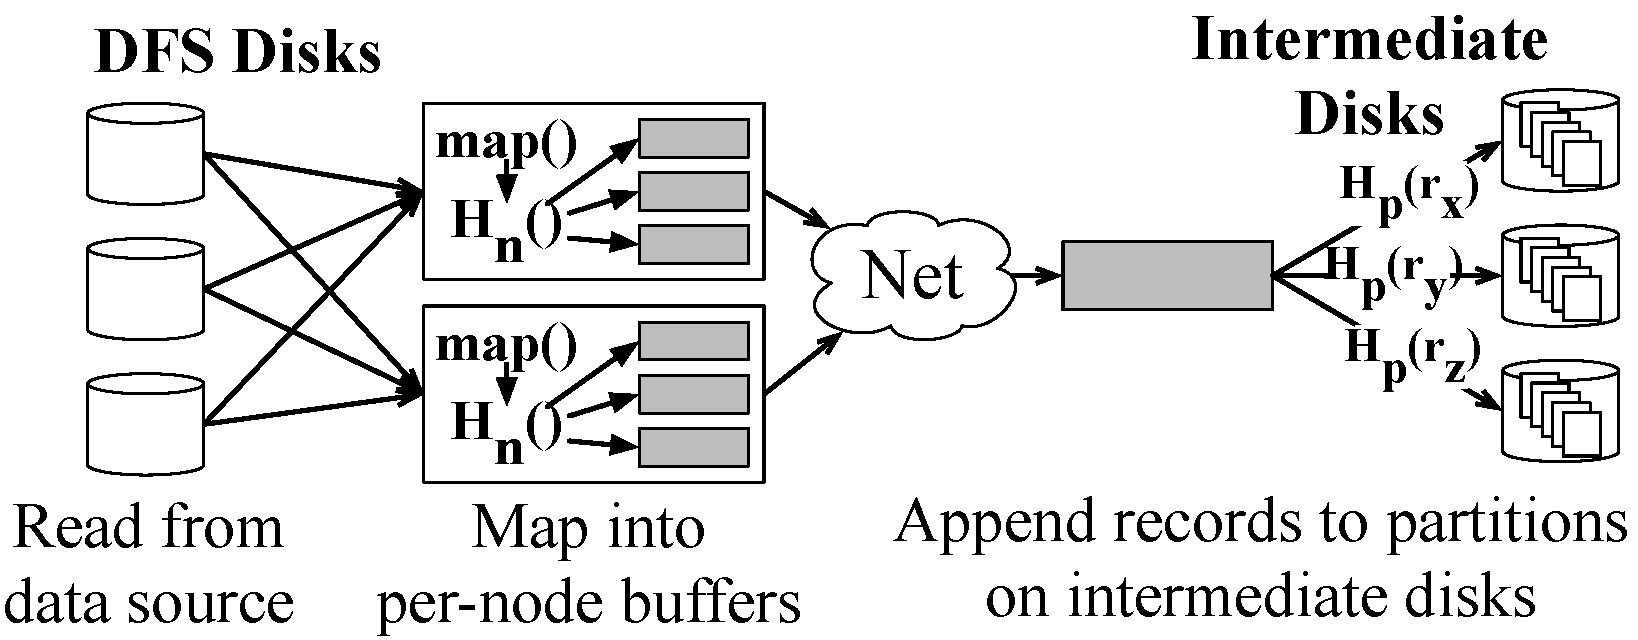
\includegraphics[width=\columnwidth]{fault_tolerance/figures/detailed_phase_one.pdf}
  \caption{\label{fig:phase_one} Phase One}
  \end{subfigure}\vspace{1em}
  \begin{subfigure}[t]{\columnwidth}
  \centering
  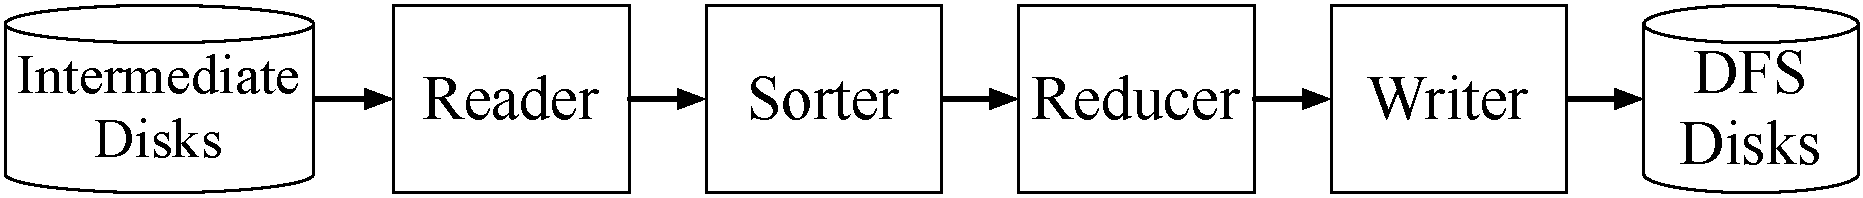
\includegraphics[width=\columnwidth]{fault_tolerance/figures/phase_two.pdf}
  \caption{\label{fig:phase_two} Phase Two}
  \end{subfigure}

  \caption{\label{fig:themis_phases} A diagrammatic overview of \themis' phases.}
\end{figure}

Nodes in a \themis cluster each have a collection of \emph{intermediate disks}
that store volatile intermediate data and a disjoint collection of \emph{DFS
  disks} that store input and output data, and are typically under the control
of a distributed file system like HDFS.

\themis runs a MapReduce job in two main \emph{phases}, called \emph{phase one}
and \emph{phase two}.  In phase one, input records are read in parallel from
the cluster's DFS disks. \themis applies the \map function to each record,
producing a collection of \emph{intermediate records} that are written to
intermediate partitions spread across the cluster's intermediate disks. Each
intermediate partition holds all records with a certain set of keys. The
mapping from keys to intermediate partitions is determined by a \emph{partition
  function}. Phase one is roughly analogous to Hadoop's map and shuffle phases.

At the end of phase one, all intermediate records have been generated,
partitioned and stored across the cluster's intermediate disks. A diagrammatic
overview of phase one is given in Figure~\ref{fig:phase_one}.

In phase two, each intermediate partition is read from the cluster's
intermediate disks completely into memory. Once in memory, it is sorted in-core
by key, and the \reduce function is applied to each group of records in the
partition with the same key. This produces a collection of \emph{output
  records} that are written to files on the DFS disks. Phase two is roughly
equivalent to Hadoop's sort and reduce phases. A diagrammatic overview of phase
two is given in Figure~\ref{fig:phase_two}.

Note that phase one requires all-to-all communication among cluster nodes, but
that phase two can be executed on each node independently.

\subsubsection{Partitioning}

In order for phase two to be processed efficiently, partitions should be small
enough for several of them to be processed in memory
simultaneously. Additionally, they should be as uniformly-sized as possible to
prevent stragglers. The partition function is responsible for ensuring both
these properties. The user can provide their own partition function, or it can
be derived at runtime through an optional sampling phase called \emph{phase
  zero}. Phase zero requires a fairly small sample to produce a good partition
function, and typically takes under a minute to run.


\subsection{Recovery Mechanism}
\label{sec:recovery}

As described in Section~\ref{fault_tolerance:sec:design}, recovering from a
failure consists of two central actions: write recovery and read recovery. In
the case of \themis, write recovery involves recovering partitions on any
intermediate disk that failed, while read recovery involves re-generating
missing pieces of partitions that a failed node should have produced, but
didn't. When a job fails, \themis will recover it by running a \emph{recovery
  job}, which is treated like a normal MapReduce job but is dedicated to
recovery.

\begin{figure}
  \centering
  \begin{subfigure}[t]{\columnwidth}
    \centering
    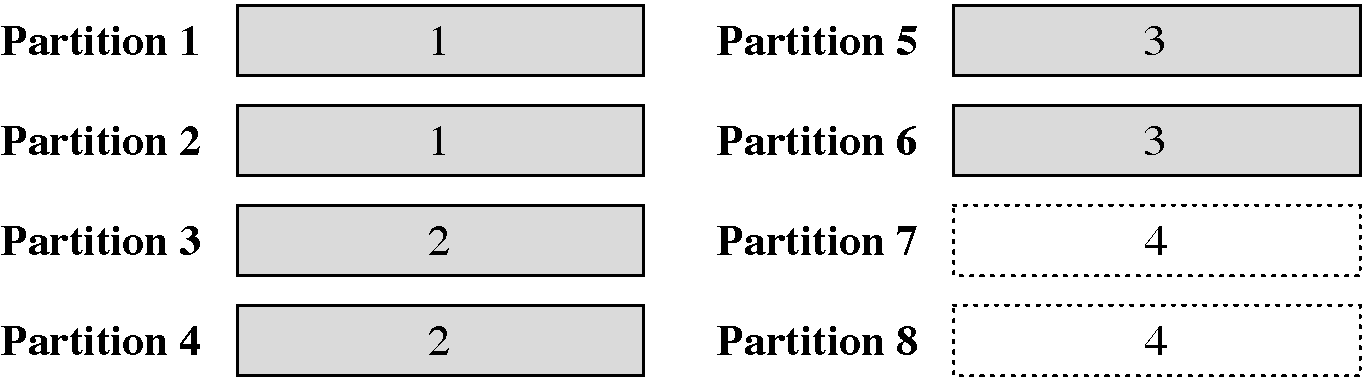
\includegraphics[width=\textwidth]{fault_tolerance/figures/disk_failure_before_recovery}
    \caption{\label{fig:disk_fail_before} The state of the job's intermediate
      partitions after the failure of disk 4. All intermediate partitions
      stored on disk 4 has been lost.}
  \end{subfigure}\hspace{0.05\textwidth}
  \begin{subfigure}[t]{\columnwidth}
    \centering
    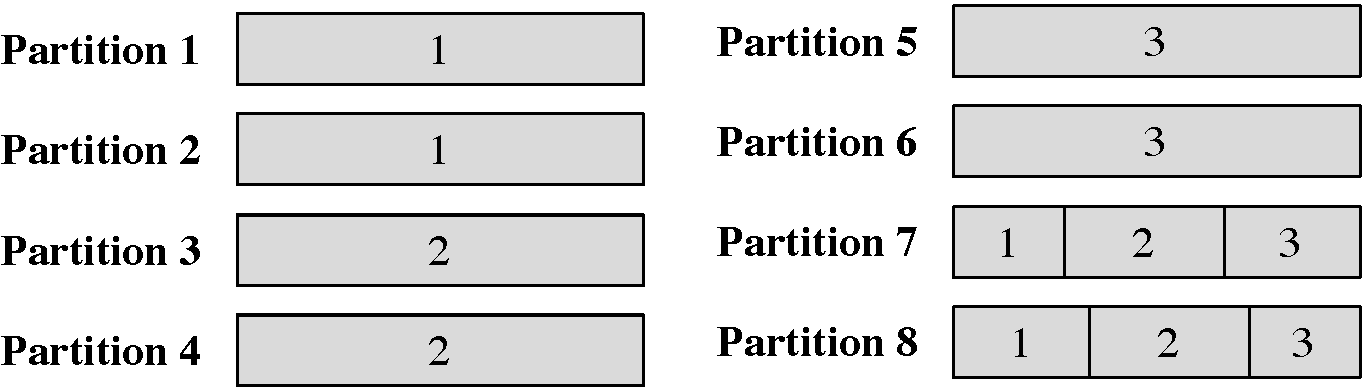
\includegraphics[width=\textwidth]{fault_tolerance/figures/disk_failure_after_recovery}
    \caption{\label{fig:disk_fail_after} The state of the job's intermediate
      partitions after recovery from the disk failure. Intermediate data for
      the partitions on disk 4 have spread across disks 1 through 3.}
  \end{subfigure}
  \caption{\label{fig:disk_fail} Illustrative example of disk failure and
    recovery in a two-node cluster with two intermediate disks per node and
    eight intermediate partitions. The rectangles
    representing each partition are labeled with the disk or disks on which
    data for that partition is stored.}
\end{figure}

Before we explore the technical details of the implementation, consider the
following illustrative example. Suppose that \themis is running on a two-node
cluster with two intermediate disks each, storing a total of eight intermediate
partitions for a particular job. In Figure~\ref{fig:disk_fail_before}, disk 4
in this cluster has failed during phase one, causing the loss of partitions 7
and 8. Figure~\ref{fig:disk_fail_after} shows the state of the intermediate
partitions at the end of phase one of the recovery job, when the data for
partitions 7 and 8 has been recovered.

Note that the recovered data for partitions 7 and 8 is spread across all the
remaining disks roughly evenly; this is highly desirable because it allows as
many disks as possible to participate in phase two of the recovery job. It
should also be noted that after the failure of disk 4 in phase one, phase two
can be run to completion on partitions 1 through 6 without waiting for the
recovery job to recover the other partitions.

\begin{figure}[t]
  \centering
  \begin{subfigure}[t]{\columnwidth}
    \centering
    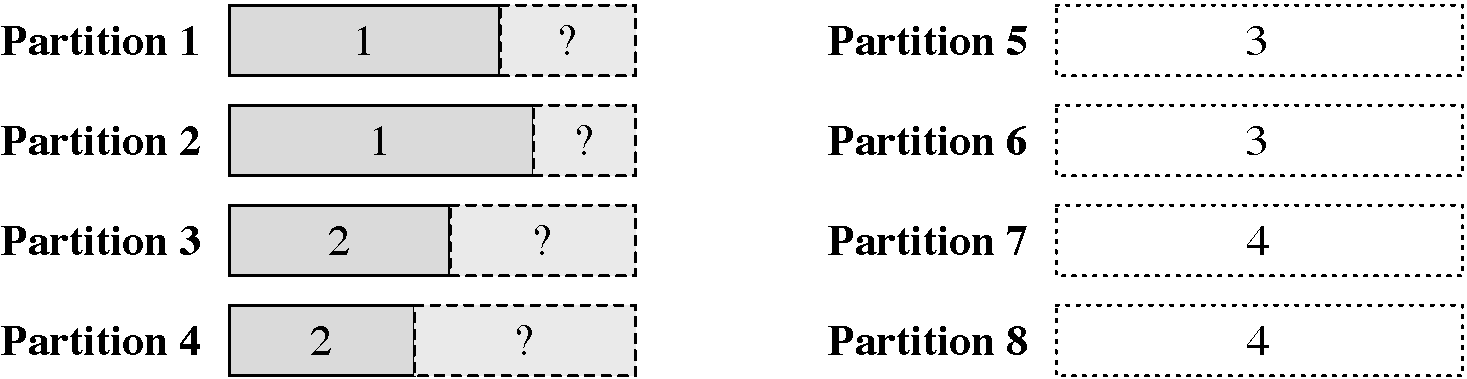
\includegraphics[width=\textwidth]{fault_tolerance/figures/node_failure_before_recovery}
    \caption{\label{fig:node_fail_before} The state of the job's intermediate
      partitions after the failure of node 2. All intermediate data for disks 3
      and 4 has been lost, and some data for the remaining partitions may not
      have been generated.}
  \end{subfigure}\hspace{0.05\textwidth}
  \begin{subfigure}[t]{\columnwidth}
    \centering
    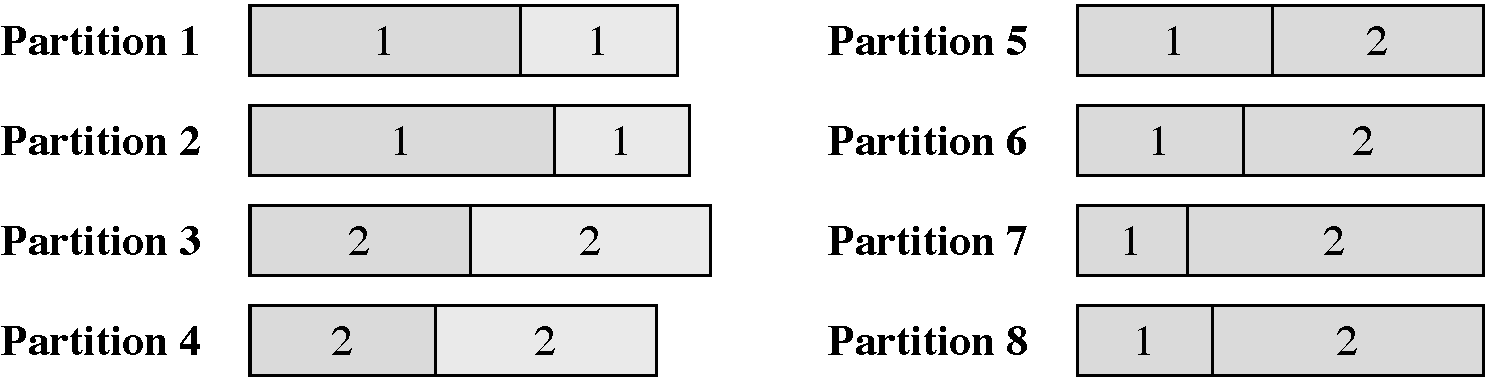
\includegraphics[width=\textwidth]{fault_tolerance/figures/node_failure_after_recovery}
    \caption{\label{fig:node_fail_after} The state of the job's intermediate
      partitions after recovery from the node failure. Intermediate data for
      the partitions on disks 3 and 4 have spread across disks 1 and 2, and
      data that should have been produced by node 2 has been added to node 1's
      partitions (although there may be duplicates).}
  \end{subfigure}
  \caption{\label{fig:node_fail} Illustrative example of node failure and
    recovery in a two-node cluster with two intermediate disks per node and
    eight intermediate partitions. A '?' indicates that it is unknown
    whether the data has been lost or not.}
\end{figure}

Figure~\ref{fig:node_fail_before} shows the same cluster after experiencing a
failure of an entire node. Not only have partitions 5 through 8 been lost, but
the remaining partitions are incomplete because the node did not finish
producing intermediate data for those partitions before it failed. Once phase
one of the recovery job has completed in Figure~\ref{fig:node_fail_after},
write recovery has spread the lost data from partitions 5 through 8 across
disks 1 and 2, while read recovery has ensured that every record that belongs
in partitions 1 through 4 has been written at least once.

\begin{table*}[t]
  \centering
  \caption{\label{table:failure_response} Table summarizing \themis' response
    to various kinds of failures at different points in the job.}
  \resizebox{\columnwidth}{!}{
  \begin{tabular}{|c|c|c|c|c|}
    \hline
    \textbf{Phase} & \textbf{Failure} & \textbf{Write Recovery} & \textbf{Read Recovery} & \textbf{Run Subsequent Phases?} \\
    \hline
    Zero (Sample) & Any & None & None & Yes \\
    One (Map + Shuffle) & Disk & Failed disk's partitions & None & Yes \\
    One (Map + Shuffle) & Node & All node's disks' partitions & Node's input files & No \\
    Two (Sort + Reduce) & Disk & Failed disk's partitions & None & Yes \\
    Two (Sort + Reduce) & Node & All node's disks' partitions & None & Yes \\
    \hline
  \end{tabular}
}
\end{table*}

In contrast to disk failure, phase two cannot be run after a node failure in
phase one because some intermediate partitions may not be complete.

If a disk or node fails in phase two, write recovery must be performed to
restore the intermediate data that was lost in the failure, but no read
recovery must be performed. Since phase zero is optional and does not produce
any output aside from a partition function, any failure during phase zero
simply requires re-executing it.

The responses to various kinds of failure in each of \themis' stages is
summarized in Table~\ref{table:failure_response}.

In the following sections, we will describe the mechanisms behind both write
and read recovery.

\subsubsection{Write Recovery}

To perform write recovery, the recovery job must re-map the failed job's input,
discarding any records that were not stored on the intermediate disks that
failed. To do this, the recovery job wraps its partition function in a
\emph{record filter}. This filter is applied to each record before it is passed
to the partition function. Abstractly, a record filter is a function that takes
a record as input and returns either ``accept'' or ``reject''. The filter
accepts a record if the record belongs to one of the partitions being
recovered, and rejects it otherwise.

In practice, \themis accomplishes record filtering in one of two ways. If the
failed job was using a user-defined partition function, the record filter
applies the failed job's partition function to the record. If the resulting
partition number is outside the range of partitions to be recovered, the filter
rejects the record.

If the original job is using a partition function generated by phase zero, the
record filter stores a set of boundary key ranges, one per contiguous range of
partitions being recovered. The complete list of boundary keys for each
partition is stored on distributed storage at the end of phase zero, and the
filter retrieves the appropriate boundary keys when it is constructed.

When an intermediate record is emitted by the \map function, the filter first
compares each intermediate record's key to the boundaries of each of its
ranges; if the record is within any of the filter's ranges, the filter
accepts the record.

In order to speed recovery by writing to as many disks in parallel as possible,
the intermediate data being recovered is spread across the cluster's remaining
intermediate disks. This is done by running phase zero during the recovery job
on a filtered sample of the input data, which generates a partition function
that spreads data in the filtered partition ranges evenly throughout the cluster.

At the end of phase one of the recovery job, any partitions that were
completely lost during a failure have been reconstituted and spread across the
cluster's remaining intermediate disks.

\subsubsection{Read Recovery}

As Table~\ref{table:failure_response} illustrates, read recovery is always
performed alongside write recovery. We take advantage of this by piggybacking
read recovery on write recovery.

In order to perform read recovery, we must first know the set of files that
were not completely processed by the failed node. \themis tracks which files
were completely mapped and received using a form of end-to-end
acknowledgments~\cite{endtoendargument}.  When a node is done reading a file in
phase one, it sends an EOF, or ``end-of-file'', annotation to every node in the
cluster indicating that the node will not receive any more data for the
file. Special care is taken to ensure that every intermediate record associated
with the file is transferred before this annotation. When a node receives an
EOF annotation, it adds the file's file ID to a list. At the end of phase one,
these lists are merged together to form a list of the nodes that received each
file. If every live node received an EOF annotation for a file, performing read
recovery on that file is not necessary. Each input file is checked for this
condition when constructing the input file list for a recovery job and files
are flagged for read recovery as appropriate.

Once phase one has completed, two sets of intermediate files will exist for the
failed job: the partially-complete set of files from the failed job and the set
of files generated as a result of read recovery. It is likely that some of the
records in these files are duplicates, and any duplicate records must be
removed to retain the \reduce function's correctness. To distinguish
intermediate records from one another, \themis tags each intermediate record
with \emph{source metadata} that uniquely identifies the record.

To uniquely identify intermediate records, we leverage the common assumption
that the \map function is deterministic and, as such, that applying the \map
function to an input record creates a totally-ordered sequence of intermediate
records. We identify an intermediate record by the position of its ``parent''
input record within the input dataset and its position in the totally-ordered
sequence of intermediate records. Specifically, we tag each record with a
64-bit file GUID, a 64-bit offset, and a 32-bit intermediate record ID. For the
purposes of evaluation, we store all 20 bytes of metadata even if the metadata
could potentially be compressed; note that for records with small offsets and
intermediate record IDs, these three pieces of metadata require far less than
20 bytes per record to store.

In phase two, intermediate partitions from the failed and recovery jobs with
the same intermediate partition number are concatenated together into an
in-memory buffer and sorted as a single intermediate partition. Before the
\reduce function is called on a set of intermediate records with a given key,
that set of records is secondarily sorted by its source metadata. The \reduce
function's record iterator then skips any records whose source metadata is the
same as that of the previous record.


\subsection{Multi-Tenancy in \themis}
\label{sec:multi-tenancy}

Each \themis node runs as a single process that assumes that it has exclusive
access to its intermediate disks and that it will not experience
memory pressure from other processes that results in swapping as long as it
does not exceed its configured memory limit. Its memory and disk management
subsystems (described in detail in~\cite{themis} and~\cite{tritonsort}) rely on
these assumptions and are the key enablers of \themis' I/O-efficiency and high
performance. Hence, running multiple \themis processes on a single node would
result in degraded performance since the processes would interfere with one
another.

\begin{figure}
  \centering
  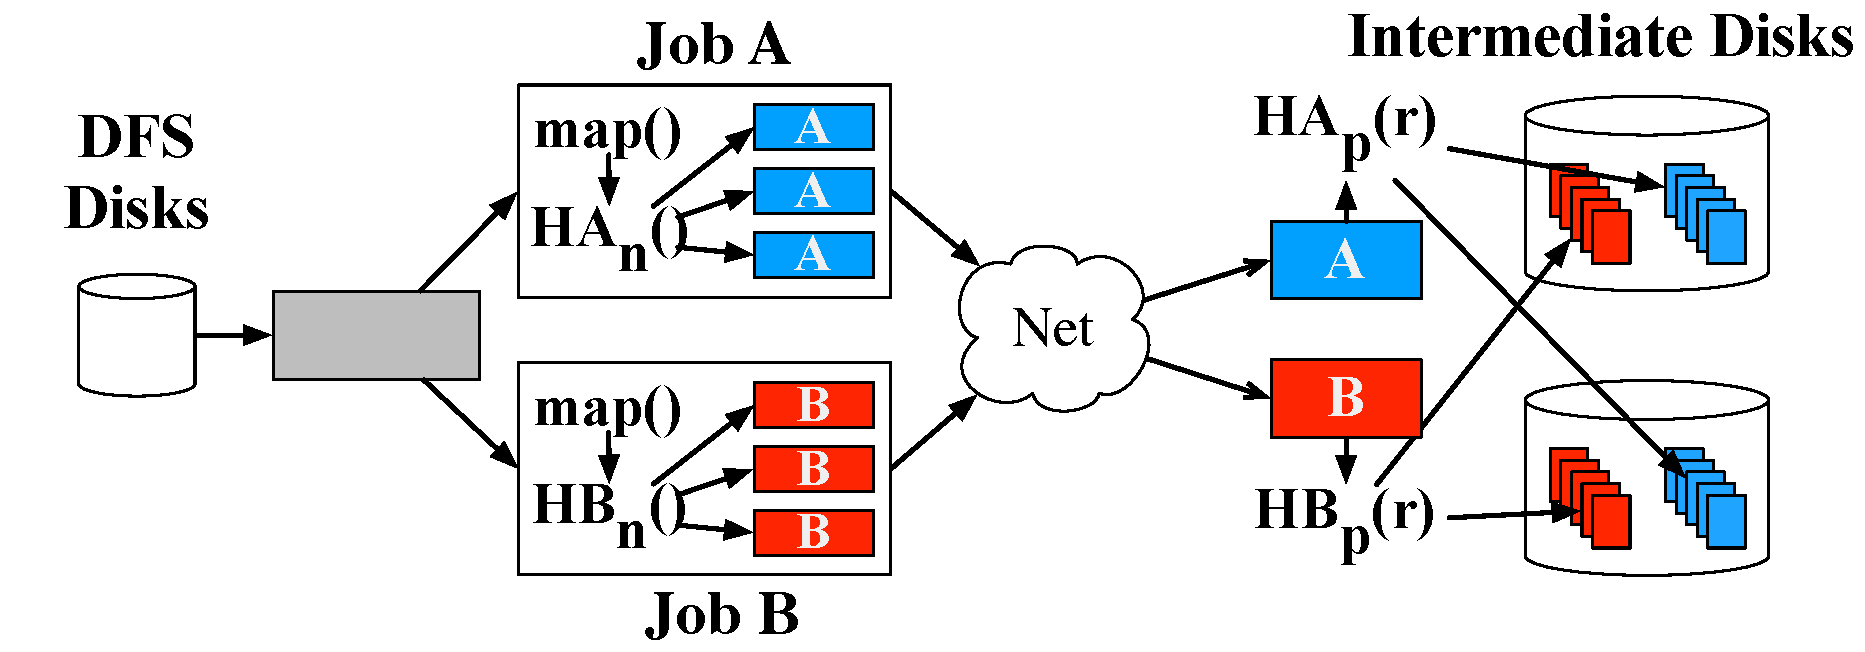
\includegraphics[width=\columnwidth]{fault_tolerance/figures/multi_tenancy}
  \caption{\label{fig:multi_tenancy} An overview of multi-tenancy in
\themis. Input records are mapped by both job A and job B's \map functions,
and intermediate records are routed based on each job's partition function independently.}
\end{figure}

To allow multiple jobs to run simultaneously in \themis with minimal
interference, we have modified \themis to support running multiple jobs
concurrently within a single process. To allow for this concurrent processing,
records read from disk are passed through each job's \map function one function
at a time, but intermediate records are transferred and written in
parallel. Buffers of intermediate records produced by a \map function are
tagged with the unique ID of that \map function's job before being sent to the
appropriate destination node. Once a buffer is received, this job ID is used to
determine to which set of intermediate partitions the buffer's records will be
written. This process is illustrated in Figure~\ref{fig:multi_tenancy}

A unique feature of our deployment prototype is that it does not co-schedule
\map and \reduce function computation. Instead, it organizes jobs into
\emph{batches}, and runs phases one and two for all jobs in a batch
simultaneously before processing the next batch. If phase zero needs to be run
to compute partition functions for any of these jobs, it is run on each job in
the batch individually before phase one starts.


\subsection{Job Dispatch}
\label{sec:control_plane}

The execution of batches of jobs is controlled by a \emph{cluster
  coordinator}. The cluster coordinator accepts descriptions of batches from
clients and coordinates their execution across the cluster's machines. Each
machine in the cluster runs a \emph{node coordinator} that is responsible for
running a \themis process on its machine and reporting an error if it crashes.

Messages are exchanged between the user, the cluster coordinator and the node
coordinators through the manipulation of message queues. Additionally, the
coordinators maintain metadata about both themselves and the jobs they run. In
our current implementation, the role of message queues and metadata store are
both filled by a Redis~\cite{redis} database. Redis was chosen primarily for
convenience; a scalable key-value store like Hyperdex~\cite{hyperdex} or
Cassandra~\cite{cassandra} and message queue like Kafka~\cite{kafka} or
Kestrel~\cite{kestrel} could be substituted.

To run a batch, the user pushes a description of the jobs in the batch to the
cluster coordinator's job queue. Upon dequeuing a batch, the cluster
coordinator assigns a unique job ID to each job in the batch. It then determines
the set of input files that each job will process, and divvies those files out
among nodes. We describe this process in more detail in
Section~\ref{sec:input_file_gathering}.


\subsection{Input Files and Distributed Storage}
\label{sec:input_file_gathering}

\begin{figure}
  \centering
  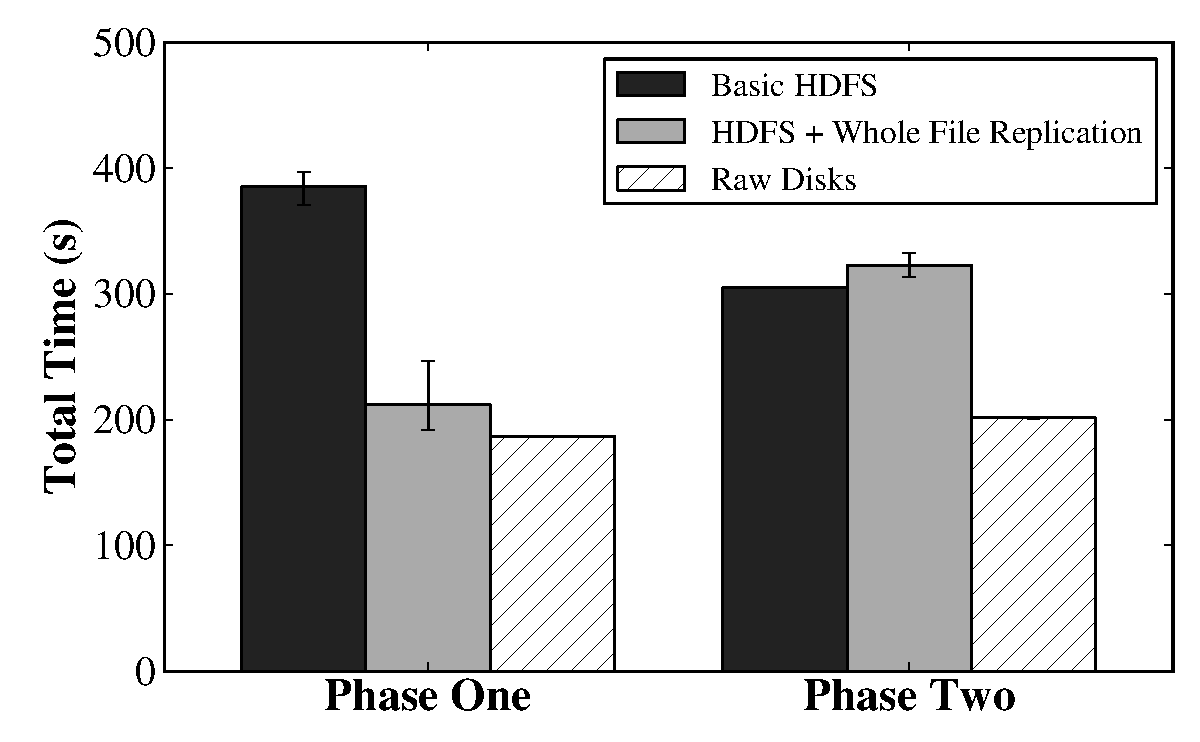
\includegraphics[width=\columnwidth]{fault_tolerance/graphs/hdfs_no_proxy_penalty}
  \caption{\label{fig:hdfs_no_proxy_penalty} Comparing the performance of
    unmodified HDFS, HDFS with whole file replication for the primary replica,
    and reading and writing from raw disks.}
\end{figure}

The specification of each \themis job includes an input directory; all files in
the input directory are processed. \themis can read input files from raw disks
or from HDFS~\cite{hdfs} using the WebHDFS REST API. We use HDFS exclusively in
this work.

Each file is uniquely identified by its URL, which is of the form\\
\texttt{<protocol>://<host>:<port>/<path from root>}. Each file is also given a
file ID that must be unique within the job. In our implementation, a
file's ID is the upper 64 bits of the MD5 hash of its URL.

Our main concern when moving from raw disks to distributed storage was
maximizing the amount of bandwidth we could achieve from the storage system.
In order to achieve sufficient bandwidth, we found that we needed to change the
way HDFS allocates blocks for files. In particular, we modified HDFS so that it
performs \emph{whole-file replication} of the file's primary replica by placing
every block on a specific disk in the cluster based on the file's name. For
example, a file named \texttt{/1.2.3.4/3/<path>} would be stored on the third
DFS disk on node \texttt{1.2.3.4}. To allow \themis to remain oblivious to this
scheme, we implemented a proxy that performs a basic round-robin allocation of
primary file replicas to cluster disks and transparently maps between regular
and placement-aware paths. The proxy only interposes itself in communication
between \themis and HDFS when a file is first opened, and imposes no additional
overhead thereafter.

Figure~\ref{fig:hdfs_no_proxy_penalty} compares the performance of an 800GB, 8
node sort with and without these modifications; as a reminder, phase one of
\themis reads sequentially from HDFS, while phase two writes sequentially to
it. The substantial performance improvement for reads is the result of the
elimination of read contention on each node's DFS disks when many files are
being read simultaneously. However, the increased rigidity of block allocation
imposed by the proxy makes the performance of writes slightly worse than
unmodified HDFS.

We found that HDFS' block placement APIs were not sufficient for providing
whole-file replication for all of a file's replicas. Hence, blocks for all
other replicas are allocated according to HDFS' default policy, and access to
non-primary replicas occurs at the speed of unmodified HDFS. The cluster
coordinator will assign files to nodes that contain their primary replica
whenever possible.


\subsection{Responding to Failures}
\label{sec:fault_response}

As node coordinators run, they refresh a keep-alive key in Redis every few
seconds; if a node fails to refresh its keep-alive key, the cluster coordinator
presumes that the node has failed. A node notifies the cluster coordinator
directly if it finds that it can no longer write to one of its intermediate
disks.

\themis attempts to insulate the rest of the cluster from a failure whenever
one occurs so that the healthy portion of the cluster can complete as much work
as possible. To avoid the attendant complexity and fragility of coordinating
failure notification across nodes, \themis simply discards any data meant for a
failed portion of the cluster. When a node fails, all existing TCP sockets to
that node will break. Nodes respond to broken sockets by discarding all data
meant for that socket for the remainder of the batch. Similarly, when a disk
fails, all data that would have been written to the failed disk for the rest of
the batch is discarded. Subsequent batches will not use failed disks or nodes
until an operator has explicitly marked them as having recovered.

Currently, the user is responsible for issuing a recovery job to recover a
failed job. Scheduling recovery jobs to maximize the likelihood of scan sharing
is beyond the scope of this work; we examine some related efforts relevant to
this problem in Chapter~\ref{chapter:related_work}.


\section{Per-Record Replay Proportionality}
\label{sec:recovery_cost}

\begin{figure}
  \centering
  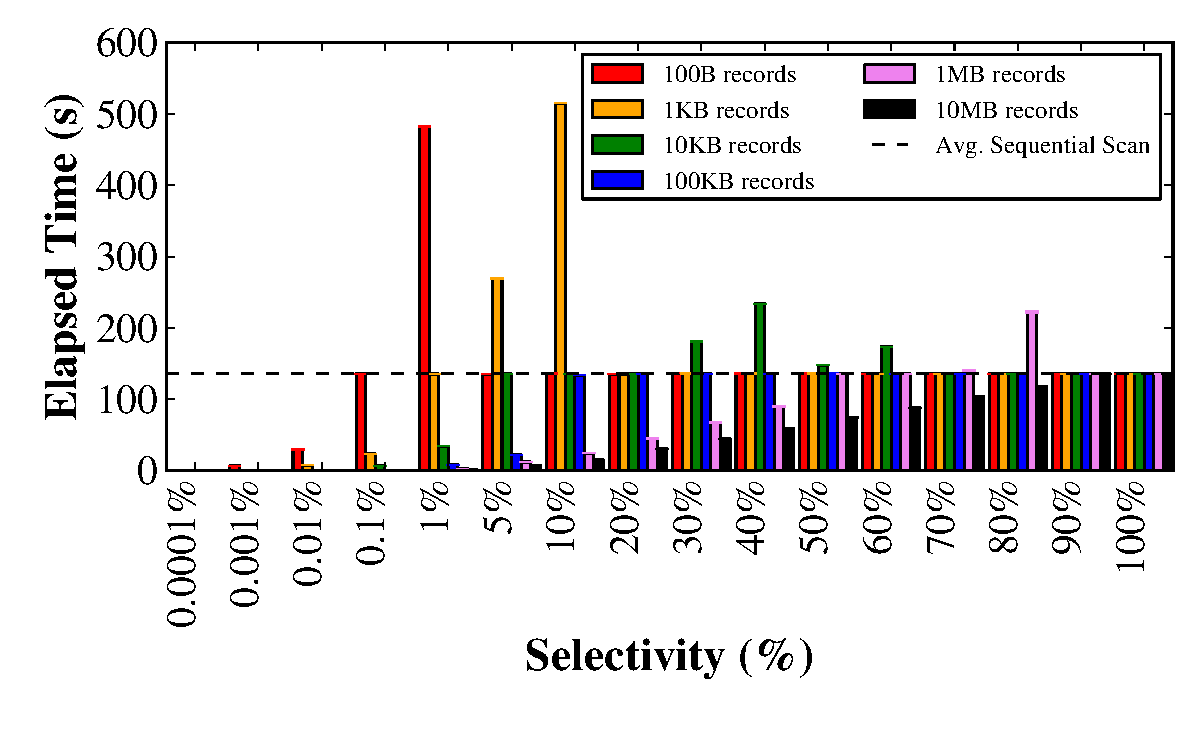
\includegraphics[width=\columnwidth]{fault_tolerance/graphs/scan_vs_seek}
  \caption{\label{fig:seek-vs-scan} Time to sequentially scan a 13.5 GB file
    vs. selectively reading a percentage of records.}
\end{figure}

\begin{figure*}
  \centering
  \begin{subfigure}[b]{\textwidth}
    \centering
    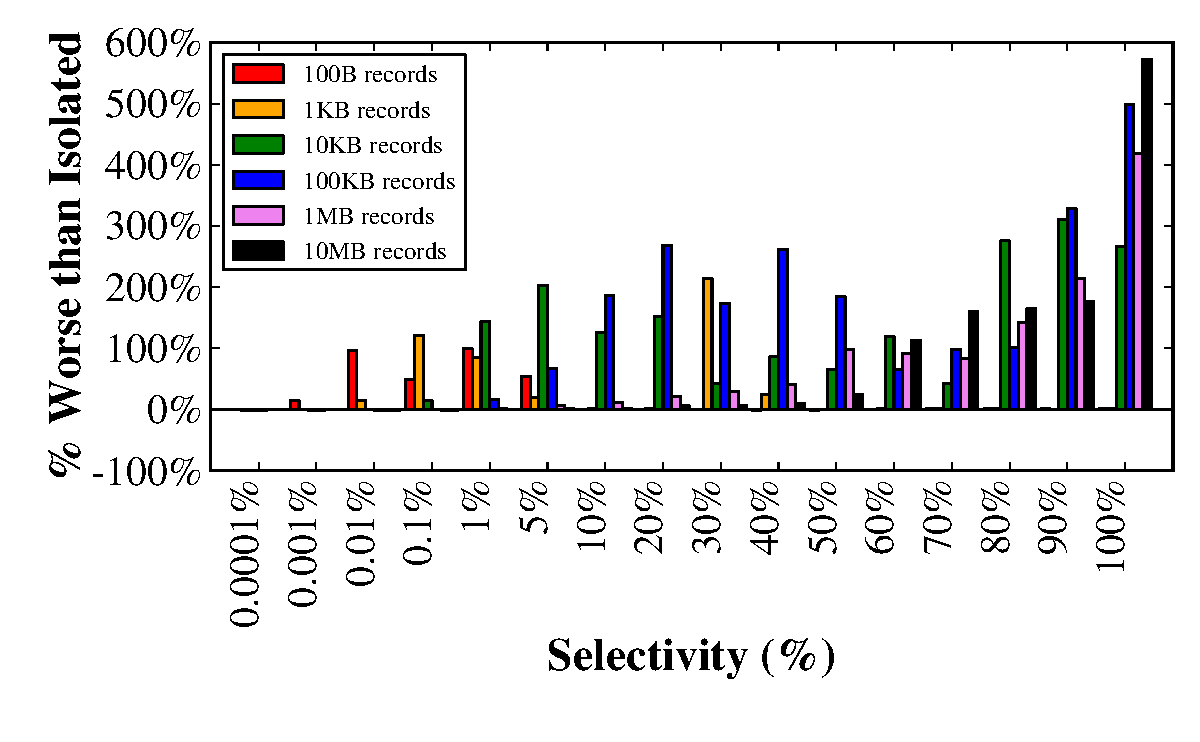
\includegraphics[width=\textwidth]{fault_tolerance/graphs/simultaneous_scan_same_file}
    \caption{\label{fig:simultaneous_same_file_scan} The effect of
      simultaneity on sequential scans.}
  \end{subfigure}
  \begin{subfigure}[b]{\textwidth}
    \centering
    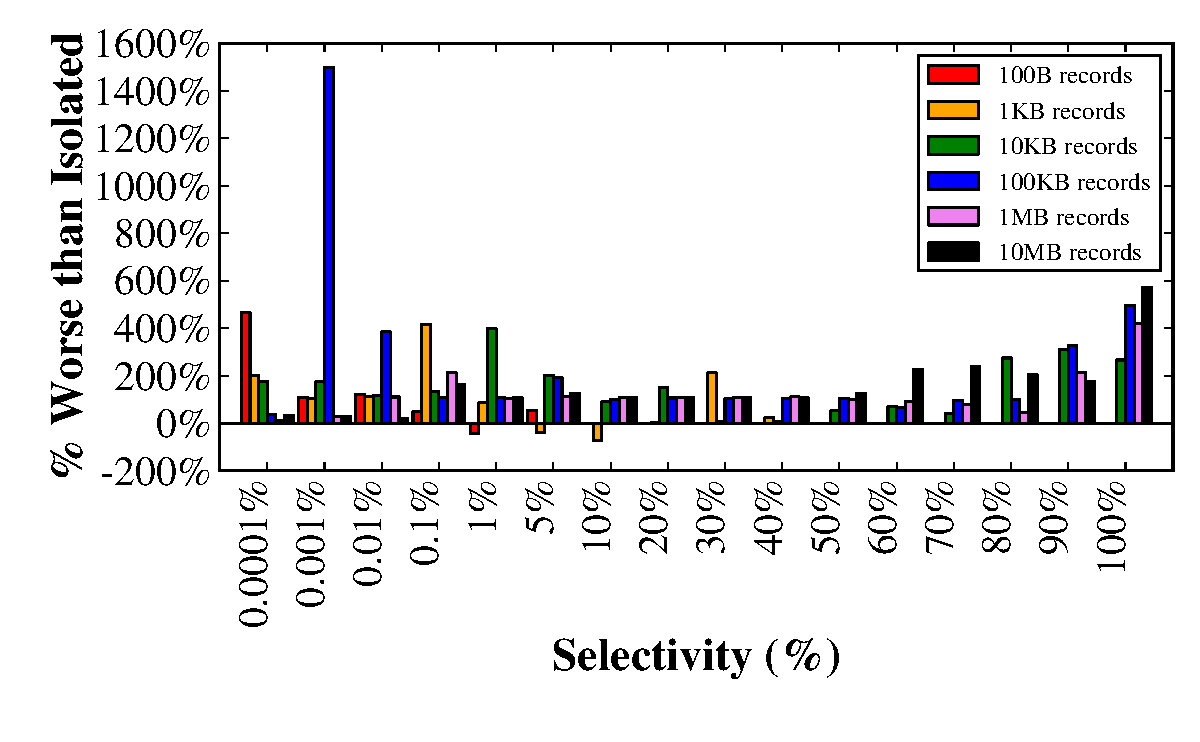
\includegraphics[width=\textwidth]{fault_tolerance/graphs/simultaneous_seek_same_file}
    \caption{\label{fig:simultaneous_same_file_seek} The effect of
      simultaneity on selective reads.}
  \end{subfigure}
  \caption{\label{fig:simultaneous_same_file} The negative impact of
    both scanning through and selectively reading from the same file simultaneously.}
\end{figure*}

\begin{figure*}
  \centering
  \begin{subfigure}[b]{\textwidth}
    \centering
    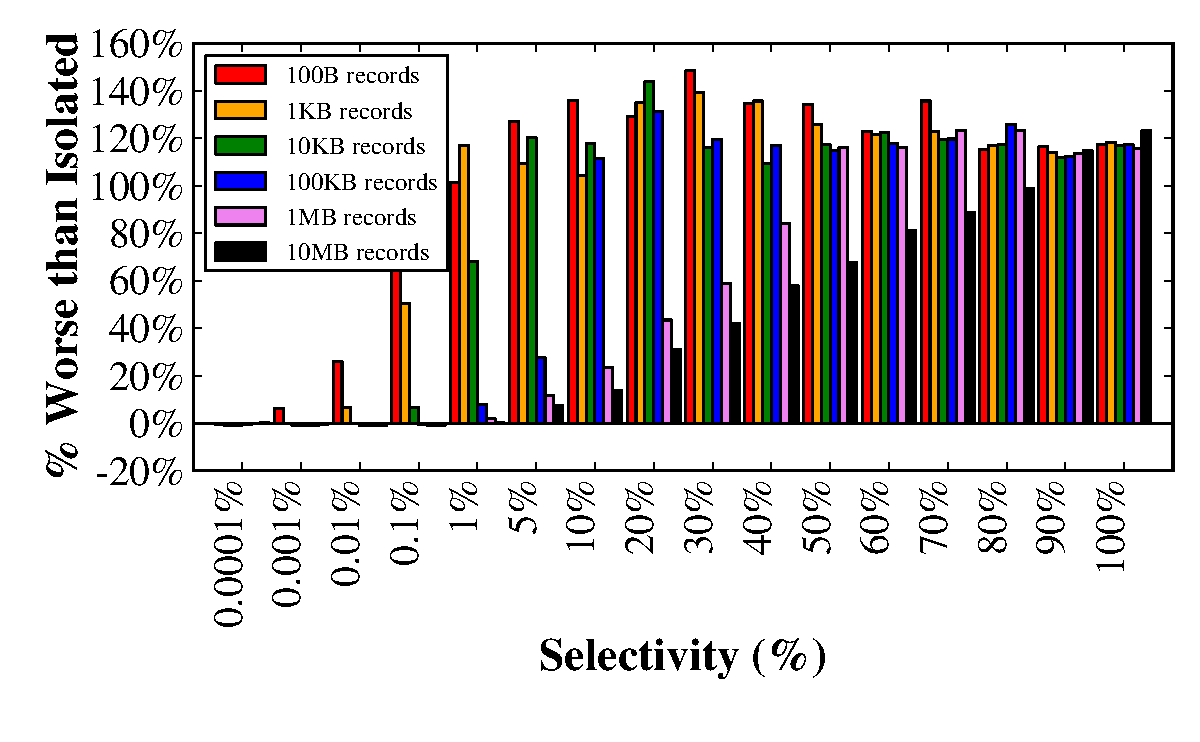
\includegraphics[width=\textwidth]{fault_tolerance/graphs/simultaneous_scan_different_files}
    \caption{\label{fig:simultaneous_different_files_scan} The effect of
      simultaneity on sequential scans.}
  \end{subfigure}
  \begin{subfigure}[b]{\textwidth}
    \centering
    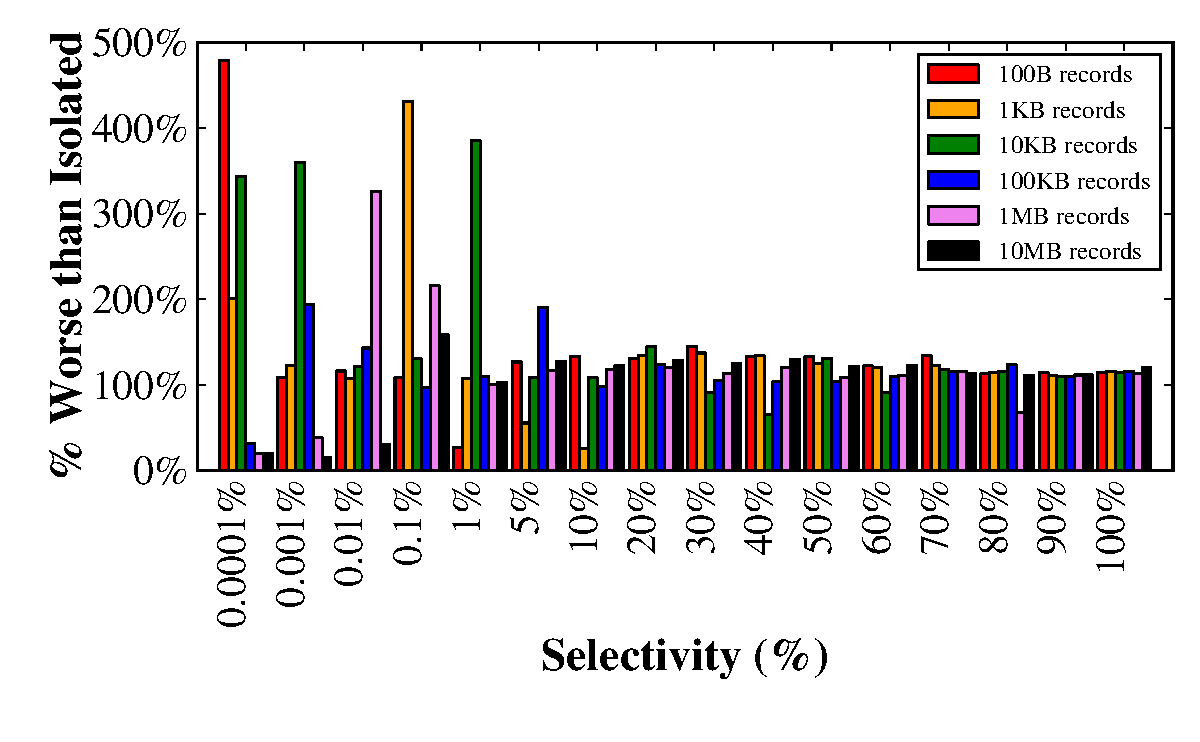
\includegraphics[width=\textwidth]{fault_tolerance/graphs/simultaneous_seek_different_files}
    \caption{\label{fig:simultaneous_different_files_seek} The effect of
      simultaneity on selective reads.}
  \end{subfigure}
  \caption{\label{fig:simultaneous_different_files} The negative impact of
    running a scan on one file while selectively reading records from a
    second file.}
\end{figure*}

When examining our options for adding fault tolerance to \themis, we were
particularly motivated by the idea of being able to recover by only reading and
re-mapping records whose intermediate data contributed to failed intermediate
partitions. We recognized that the overhead of storing this information would
potentially be quite high; in general, it requires storing information about
the lineage and intermediate partition of every intermediate
record. Nonetheless, we wanted to gain an understanding of the regimes in which
this overhead might be a reasonable tradeoff for a decreased recovery time. In
this section, we examine the potential benefits and disadvantages of this
approach using a microbenchmark.

To evaluate the potential time savings from selectively reading the subset of
input records needed to perform recovery, we created a 13.5 GB file on one of
our cluster's disks and compared the time taken to completely scan through the
file with the time taken to read a certain percentage of the file's
records. The percentage of records selectively read roughly corresponds to the
``selectivity'' of the recovery being simulated. For example, if 1\% of records
are being read, this corresponds to the amount of reading necessary to recover
from a lost of 1\% of the cluster's intermediate partitions.

As a simplifying assumption, we assumed that the records are evenly spaced
throughout the file. We completely purged the operating system's file buffer
cache and disabled any caching on our disk controllers so that each experiment
started from a cold cache.

As Figure~\ref{fig:seek-vs-scan} shows, when the selectivity of recovery is
quite small, selective reads can achieve large speedups over a sequential
scan. However, selectively reading records is far from proportional. For
example, for a file with 1KB records, the cost of sequentially scanning the
file is the same as the cost of selectively reading 1\% of its records; this
means that the loss of more than 1\% of the cluster's intermediate partitions
can be recovered from just as quickly by scanning input files as it can by
selectively reading them for I/O-bound jobs.

We suspect that this non-proportionality is due to a combination of the
overhead of seeking between records, the overhead of the relatively many
\texttt{read()} syscalls needed to retrieve those records, and the behavior of
the operating system's buffer cache. Note that for certain record sizes and
selectivities, selective reading performs dramatically worse than sequential
scanning; this is due mainly to poor interaction between the application and
the buffer cache.

In addition to its non-proportionality, selective reads have a negative impact
on the performance of other concurrent operations to the same
disk. Figure~\ref{fig:simultaneous_same_file} shows that selectively reading
from a file while scanning through it simultaneously can decrease the speed of
the scan by up to 600\%. We believe that cache interference between the two
writing processes, as well as the mechanical act of disrupting the sequentiality
of disk access with seeking, are the source of these overheads.

Figure~\ref{fig:simultaneous_different_files} shows the impact of running a
scan and a selective read over two different files on the same disk
simultaneously. Here the performance decrease for scans is much less drastic;
we believe the primary source of this performance decrease to be the overhead
imposed on the scan by disk seeks.

These results indicate, somewhat intuitively, that when the selectivity of the
recovery is very small (less than 0.01\%), it is highly beneficial to perform
selective reads. However, selective reads are only a proportional form of fault
tolerance if records are relatively large, and they have the potential to
interact poorly with other concurrent sequential scans. In addition, a recovery
with small selectivity is only likely when the cluster is fairly large, which
is a different operating environment from the ``dense'' clusters on which we
focus in this work.

\section{Evaluation}
\label{fault_tolerance:sec:eval}

In Section~\ref{fault_tolerance:sec:methodology}, we describe our experimental methodology. In
Section~\ref{sec:proportionality}, we show that recovery from both disk and
node failure are proportional, in that the time taken to recover is
proportional to the size of the failure. In
Section~\ref{sec:scan_sharing_overhead}, we show that the overhead imposed by
scan sharing a normal job with a recovery job is low.

\subsection{Methodology}
\label{fault_tolerance:sec:methodology}

We evaluated our fault tolerance mechanisms on eight of the machines in the
cluster described in Section~\ref{sec:hardware_architecture}. Each hard drive
is configured with a single XFS partition that is configured with a single
allocation group to avoid file fragmentation across allocations groups and is
mounted with the \texttt{noatime}, \texttt{nobarrier} and \texttt{noquota}
flags set. For this evaluation, all servers were running Linux 2.6.32. Jobs
source and sink data to HDFS, configured with 128MB blocks and whole-file
replication of the primary replica of each file.

\themis is written in C++ and, in this evaluation, is compiled with
\texttt{g++} 4.7.1. The cluster coordinator, node coordinator and HDFS
rewriting proxy are written in Python.

We rely on the sort MapReduce job to evaluate our fault tolerance
mechanisms. Since sort corresponds to no-op \map and \reduce functions, it
provides a natural way of evaluating fault tolerance independently of the job
being performed. At the same time, sort's large intermediate data set size
allowed us to stress-test the system's ability to scale
proportionally. Additionally, we have found it logistically difficult to both
obtain and store freely-available data sets that are sufficiently large that
they do not fit in a single node's memory. The input data set for sort is easy
to generate synthetically, which allows us to scale the evaluation beyond a
single node.

\subsection{Proportionality of Recovery}
\label{sec:proportionality}

In this section, we explore the proportionality of our recovery process in
response to disk and node failures.

\subsubsection{Recovering From Disk Failure}
\label{sec:disk_proportionality}

\begin{figure}
  \centering
  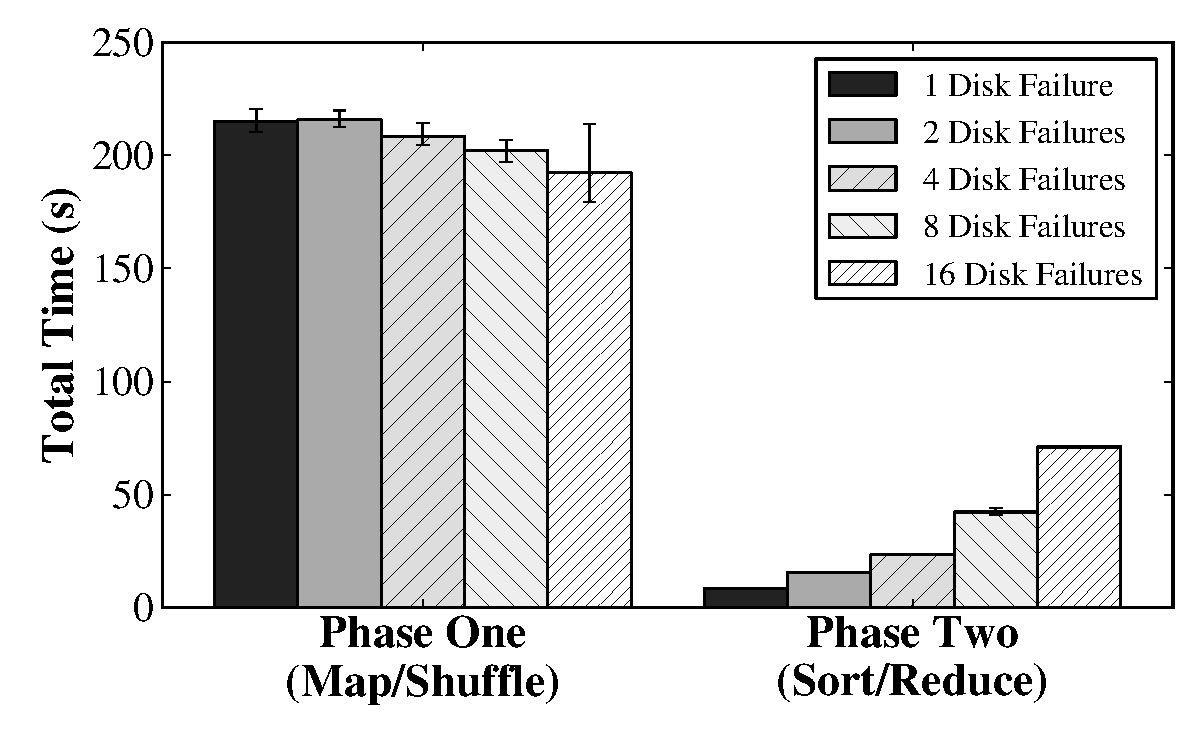
\includegraphics[width=\columnwidth]{fault_tolerance/graphs/disk_recovery_proportionality.pdf}
  \caption{\label{fig:disk_recovery_proportionality} Runtime of recovery from a
    disk failure during an 800GB sort with an increasing number of failed
    disks.}
\end{figure}

To test the proportionality of recovery from a disk failure, we ran an 800GB
sort job across our eight-node testbed and failed an increasing number of disks
during phase one. Disk failures were injected into the system by making the
part of \themis that writes to intermediate disks fail after it had written a
certain number of bytes to the disks we wanted to fail. We then ran a recovery
job to recover the data from those failed
disks. Figure~\ref{fig:disk_recovery_proportionality} shows the elapsed time of
both phases for the recovery job.

The elapsed time of the recovery job's phase two increases sub-linearly as the
number of disk failures increases.  This is because phase two is designed to
process multiple intermediate partitions in parallel and the number of
partitions created during recovery is fairly small, so processing twice as many
partitions doesn't necessarily take twice as much time. The decrease in phase
one's recovery time as the number of disks to recover increases is coincidental
and simply reflects the variability of access time provided by HDFS.

\subsubsection{Recovering From Node Failure}

\begin{figure}
  \centering
  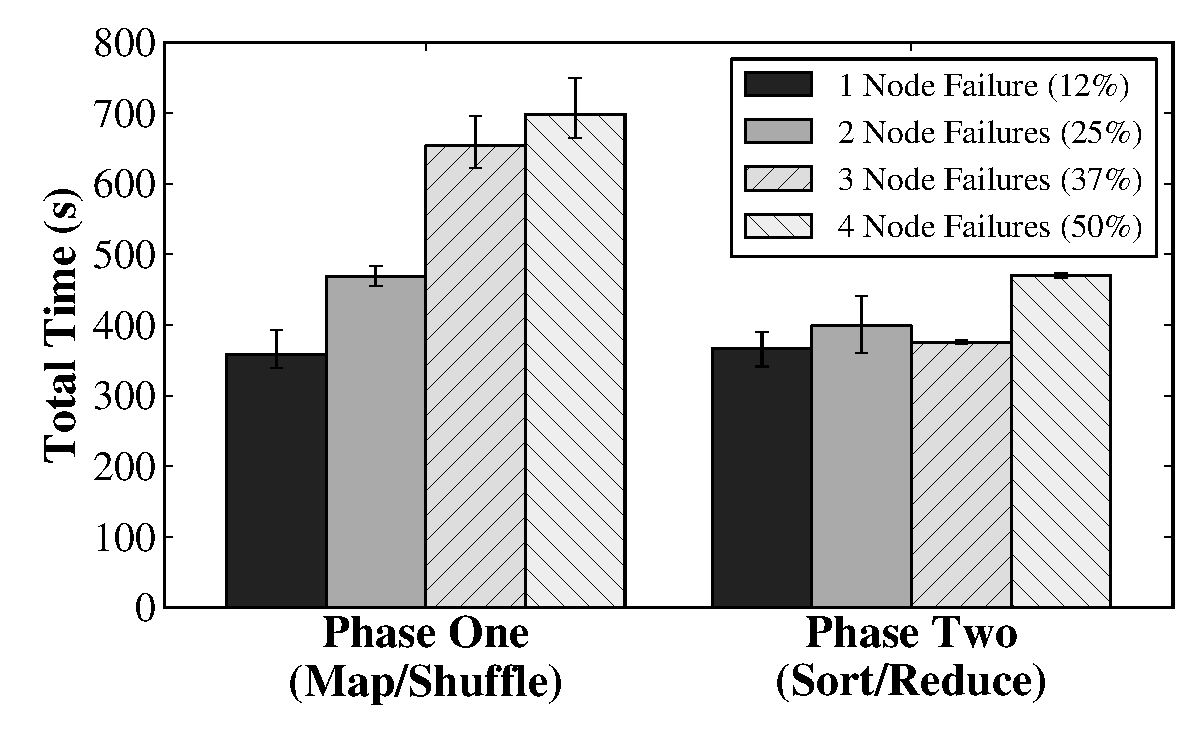
\includegraphics[width=\columnwidth]{fault_tolerance/graphs/node_recovery_proportionality.pdf}
  \caption{\label{fig:node_recovery_proportionality} Runtime of recovery from
    node failures during an 800GB sort.}
\end{figure}

To test the proportionality of recovery from node failure, we ran the same
800GB sort job as in the disk failure tests, but instead of failing individual
disks, we killed all \themis-related processes on a set of nodes approximately
120 seconds after starting the job. Each DFS disk's input consists of ten
evenly-sized files, each approximately 1.6GB
long. Figure~\ref{fig:node_recovery_proportionality} shows the elapsed time of
both phases of the recovery jobs for these failures.

Phase one's recovery time increases drastically as the number of failures
increase. The primary reason for this is that the same amount of recovery must
be done across an increasingly small number of nodes. Recovery time in phase
one is further increased by the fact that nodes are typically not accessing the
whole-file-replicated primary replica of the files they are recovering; as a
result, read performance degrades to that of unmodified HDFS.

Phase two's recovery time increases sub-linearly for the same architectural
reasons that it increases sub-linearly during disk recovery. Due to end-of-file
acknowledgments, only a small number of duplicate records are generated. As a
result, phase two's node recovery is roughly equivalent to scan-sharing phase
two of a normal 800GB sort with a disk recovery for all of the failed nodes'
disks.

\begin{figure}[t]
  \centering
  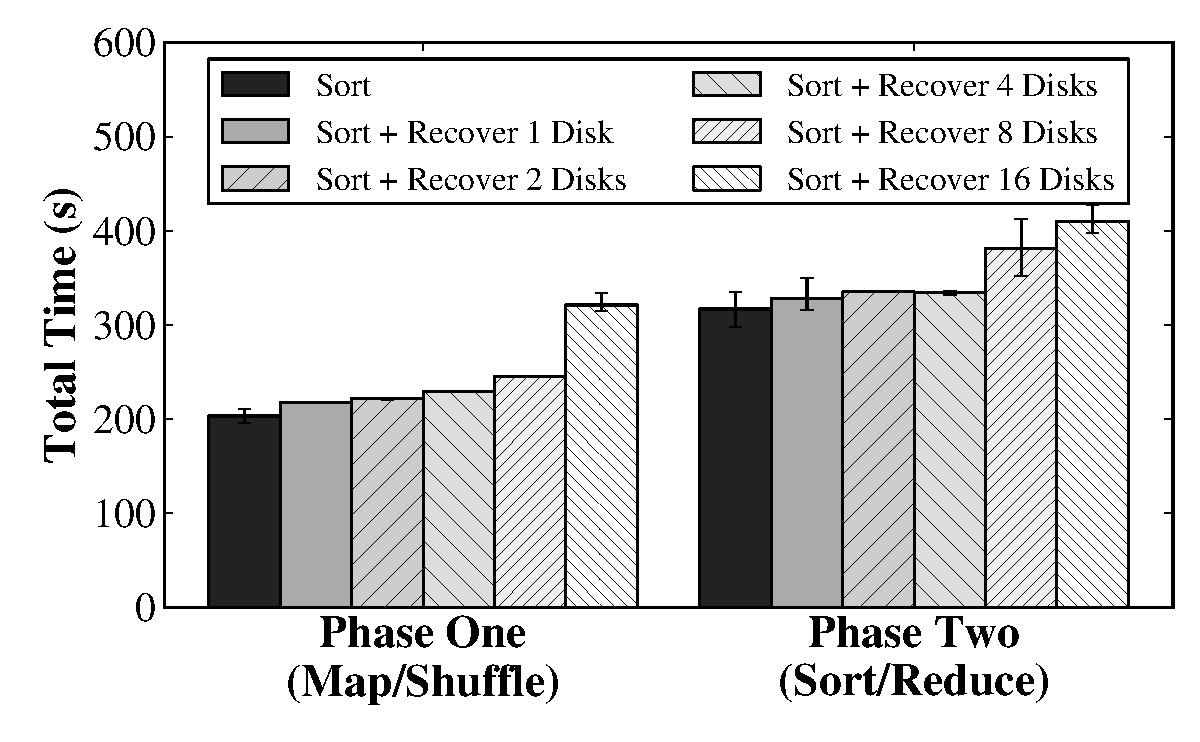
\includegraphics[width=\columnwidth]{fault_tolerance/graphs/scan_share_overhead.pdf}
  \caption{\label{fig:scan_sharing_overhead} Comparing the baseline performance
    of an 800GB sort with the performance of scan-sharing that sort with disk
    failure recovery jobs.}
\end{figure}

\subsection{Scan Sharing Overhead}
\label{sec:scan_sharing_overhead}

To evaluate the overhead imposed on a normal job by scan-sharing it with a
recovery job, we ran an 800GB sort job scan-shared with the recovery jobs
described in Section~\ref{sec:disk_proportionality}. In
Figure~\ref{fig:scan_sharing_overhead}, we see that phase one's runtime remains
fairly flat until we scan-share the sort job recovery of eight disks. At this
point, the system is writing so much intermediate data to the remaining disks
that it transitions from being bound by the speed at which it can read from
HDFS to being bound by the speed at which it can write to its intermediate
disks. At the same time, the amount of intermediate data produced by the
recovery job becomes large enough to visibly impact phase two.

\section{Conclusions}

MapReduce's traditional approach to fault tolerance is proportional, but it
imposes the overhead of additional rounds of I/O in common-case operation,
which negatively impacts the system's overall performance. In this work, we
have shown that, through leveraging the multi-tenancy typical of a MapReduce
cluster and composing previously-known fault tolerance techniques, it is
possible to provide proportional fault tolerance without imposing additional
rounds of I/O in failure-free operation.

\section{Acknowledgments}

This work was sponsored in part by NSF Grants CSR-1116079 and MRI CNS-0923523,
and through donations by Cisco Systems and a NetApp Faculty Fellowship.

Chapter~\ref{chapter:fault_tolerance} contains material as it appears in the
Proceedings of the ACM Symposium on Cloud Computing (SOCC) 2012. Rasmussen,
Alexander; Porter, George; Vahdat, Amin. The dissertation author was the
primary investigator and author of this paper.

Chapter~\ref{chapter:fault_tolerance} contains material submitted for
publication as ``I/O-Efficient Fault Tolerance for MapReduce''. Rasmussen,
Alexander; Porter, George; Vahdat, Amin. The dissertation author was the
primary investigator and author of this paper.


